\chapter{Temporal disaggregation}
\label{chap:tdisagg}

\newcommand{\Yb}{\mathbf{Y}}
\newcommand{\Xb}{\mathbf{X}}
\newcommand{\CXb}{\mathbf{CX}}
\newcommand{\Cb}{\mathbf{C}}
\newcommand{\Vb}{\mathbf{V}}
\newcommand{\Db}{\mathbf{D}}

\def\tditem[#1]#2{\item[{\tt #1}]#2}

\section{Introduction}
\label{sec:tdisagg-intro}

This chapter describes and explains the facility for temporal
disaggregation in gretl.\footnote{We are grateful to Tommaso Di Fonzo
for detailed and precise comments on earlier drafts. Any remaining
errors are, of course, our responsibility.} This is implemented by the
\texttt{tdisagg} function, which supports three variants of the method
of \cite{chowlin71}; the method of \cite{fernandez81}; and two
variants of the method of \cite{denton71} as modified by
\cite{cholette84}. Given the analytical similarities between them, the
three Chow--Lin variants and the Fern\'andez method will be grouped in
the discussion as below ``Chow--Lin methods''.

The balance of this section provides a gentle introduction to the idea
of temporal disaggregation; experts may wish to skip to the next
section.

Basically, temporal disaggregation is the business of taking
time-series data observed at some given frequency (say, annually) and
producing a counterpart series at a higher frequency (say,
quarterly). The term ``disaggregation'' indicates the inverse
operation of aggregation, and to understand temporal disaggregation
it's helpful first to understand temporal aggregation. In aggregating
a high frequency series to a lower frequency there are three basic
methods, the appropriate method depending on the nature of the data.
Here are some illustrative examples.
\begin{itemize}
\item GDP: say we have quarterly GDP data and wish to produce an
  annual series. This is a \textit{flow variable} and the annual flow
  will be the \textit{sum} of the quarterly values (unless the
  quarterly values are annualized, in which case we would aggregate by
  taking their their mean).
\item Industrial Production: this takes the form of an \textit{index}
  reporting the level of production over some period relative to that
  in a base period in which the index is by construction 100. To
  aggregate from (for example) monthly to quarterly we should take the
  \textit{average} of the monthly values. (The sum would give a
  nonsense result.) The same goes for price indices, and also for
  ratios of stocks to flows or vice versa (inventory to sales, debt to
  GDP, capacity utilization).
\item Money stock: this is typically reported as an
  \textit{end-of-period} value, so in aggregating from monthly to
  quarterly we'd take the value from the final month of each
  quarter. In case a stock variable is reported as a
  \textit{start-of-period} value, the aggregated version would be that
  of the first month of the quarter.
\end{itemize}

A central idea in temporal disaggregation is that the high frequency
series must respect both the given low frequency data and the
aggregation method. So for example, whatever numbers we come up with
for quarterly GDP, given an annual series as starting point, our
numbers must sum to the annual total. If money stock is measured at
the end of the period then whatever numbers we come up with for
monthly money stock, given quarterly data, the figure for the last
month of the quarter must match that for the quarter as a whole.  This
is why temporal disaggregation is sometimes called ``benchmarking'':
the given low frequency data constitute a benchmark which the
constructed high frequency data must match, in a well defined sense
that depends on the nature of the data.

Colloquially, we might describe temporal disaggregation as
``interpolation,'' but strictly speaking interpolation applies only to
stock variables. We have a known end-of-quarter value (say), which is
also the value at the end of the last month of the quarter, and we're
trying to figure out what the value might have been at the end of
months 1 and 2. We're filling in the blanks, or interpolating. In the
GDP case, however, the procedure is \textit{distribution} rather than
interpolation. We have a given an annual total and we're trying to
figure out how it should be distributed over the quarters. We're also
doing distribution for variables taking the form of indices or ratios,
except in this case we're seeking plausible values whose mean equals
the given low-frequency value.

While matching the low frequency benchmark is an important constraint,
it obviously does not tie down the high frequency values. That is a
job for either regression-based methods such as Chow--Lin or
non-regression methods such as Denton. Details are provided in
section~\ref{sec:tdisagg-details}.

\section{Notation and design}
\label{sec:tdisagg-nd}

Some notation first: the two main ingredients in temoral
disaggregation are
\begin{itemize}
\item a $T \times g$ matrix $\Yb$ (holding the series to be
  disaggregated) and
\item a matrix $\Xb$ with $k$ columns and $(s \cdot T + m)$ rows (to
  aid in the disaggregation).
\end{itemize}
The idea is that $\Yb$ contains time series data sampled at some
frequency $f$, while each column of $\Xb$ contains time series data at
a higher frequency, $sf$. So for each observation $Y_t$ we have $s$
corresponding rows in $\Xb$. The object is to produce a transformation
of $\Yb$ to frequency $sf$, with the help of $\Xb$ (whose columns are
typically called ``related series'' or ``indicators'' in the temporal
disaggregation literature), via either distribution or interpolation
depending on the nature of the data. For most of this document we will
assume that $g = 1$, or in other words we are performing temporal
disaggregation on a single low-frequency series, but \texttt{tdisagg}
supports ``batch processing'' of several series and we return to this
point in section~\ref{sec:tdisagg-multi}.

If the $m$ in $(s \cdot T + m)$ is greater than zero, that implies
that there are some ``extra'' high-frequency observations available
for extrapolation. The output of the function will therefore have as
many rows as $\Xb$, including $m$ forecasts if applicable.

We need to say something more about what goes into $\Xb$. Under the
Denton methods this must be a single series, generally known as the
``preliminary series''.\footnote{There's nothing to stop a user from
  \textit{constructing} such a series using several primary series as
  input---by taking the first principal component or some other
  means---but that possibility is beyond our scope here.} For the
Chow--Lin methods, $\Xb$ can hold a combination of deterministic terms
(e.g.\ constant, trend) and stochastic series. Naturally, suitable
candidates for the role of preliminary series or indicator will be
variables that are correlated with $\Yb$ (and in particular, might be
expected to share short-run dynamics with $\Yb$). However, it is
possible to carry out disaggregation using deterministic terms
only---in the simplest case, with $\Xb$ containing nothing but a
constant. Experts in the field tend to frown on this, with reason: in
the absence of any genuine high-frequency information disaggregation
just amounts to a ``mechanical'' smoothing. But some people may have a
use for such smoothing, and it's permitted by \texttt{tdisagg}.

In light of the foregoing, we should draw attention to a design
decision in \texttt{tdisagg}: we have separated the specification of
indicators in $\Xb$ from certain standard deterministic terms that
might be wanted, namely, a constant, a linear trend and a quadratic
trend. This means that if you want a disaggregation \textit{without}
stochastic indicators, you can omit (or set to \texttt{null}) the
argument corresponding to $\Xb$. In that case a constant (only) will
be employed automatically, but for the Chow--Lin methods one can
adjust the deterministic terms used via an option named \texttt{det},
described below. In other words the content of $\Xb$ becomes
implicit. See section~\ref{sec:tdisagg-det} for more detail.

Here's an important point to note when $\Xb$ is given explicitly:
although this matrix may contain extra observations ``at the end'' we
assume that $\Yb$ and $\Xb$ are \textit{correctly aligned at the
  start}. Take for example the annual to quarterly case: if the first
observation in annual $\Yb$ is for 1980 then the first observation in
quarterly $\Xb$ must be for the first quarter of 1980. Ensuring this
is the user's responsibility. We will have some more to say about this
in the following section.

\section{Overview of data handling}
\label{sec:tdisagg-data}

The \texttt{tdisagg} function has three basic arguments, representing
$\Yb$, $\Xb$ and $s$ respectively (plus several options; see
below). The first two arguments can be given either in matrix form as
such, or as ``dataset objects''---that is, a series for $\Yb$ and a
series or list of series for $\Xb$. Or, as mentioned above, $\Xb$ can
be omitted (left implicit). This gives rise to five cases; which is
most convenient will depend on the user's workflow.

\begin{enumerate}
\item Both $\Yb$ and $\Xb$ are matrices. In this case, the size and
  periodicity of the currently open dataset (if any) are irrelevant.
  If $\Yb$ has $T$ rows $\Xb$ must, of course, have at least
  $s \cdot T$ rows; if that condition is not satisfied an ``Invalid
  argument'' error will be flagged.
\item $\Yb$ is a series (or list) and $\Xb$ a matrix. In this case we
  assume that the periodicity of the currently open dataset is the
  \emph{lower} one, and $T$ will be taken as equal to \texttt{\$nobs}
  (the number of observations in the current sample range). Again,
  $\Xb$ must have at least $s \cdot T$ rows.
\item $\Yb$ is a matrix and $\Xb$ a series or list.  We then assume
  that the periodicity of the currently open dataset is the
  \emph{higher} one, so that \texttt{\$nobs} defines
  ($s \cdot T + m$). And $\Yb$ is supposed to be at the lower
  frequency, so its number of rows gives $T$. We should then be able
  to find $m$ as \texttt{\$nobs} minus $s \cdot T$; if $m < 0$ an
  error is flagged.
\item Both $\Yb$ and $\Xb$ are ``dataset objects''.  We have two
  sub-cases here.
  \begin{enumerate}
  \item If $\Xb$ is a series, or an ordinary list of series, the
    periodicity of the currently open dataset is taken to be the
    \emph{higher} one. The series (or list) containing $\Yb$ should
    hold the appropriate entries \emph{every $s$ elements}. For
    example, if $s = 4$, $Y_1$ will be taken from the first
    observation, $Y_2$ from the fifth, $Y_3$ from the ninth, and so
    on. In practical terms, series of this sort are likely to be
    composed by repeating each element of a low-frequency variable $s$
    times.
  \item Alternatively, $\Xb$ could be a ``MIDAS list''. The concept of
    a MIDAS list is fully explained in
    chapter~\ref{chap:mixed-frequency} but for example, in a quarterly
    dataset a MIDAS list would be a list of three series, for the
    third, second and first month (note the ordering). In this case,
    the current periodicity is taken to be the \emph{lower} one and
    $\Xb$ will contain one column, corresponding to the high-frequency
    representation of the MIDAS list.
  \end{enumerate}
\item $\Xb$ is omitted. If $\Yb$ is given as a matrix it is taken to
  have $T$ rows. Otherwise the interpretation is determined
  heuristically: if the $\Yb$ series is recognized by gretl as
  composed of repeated low-frequency observations, or if a series
  result is requested, it is taken as having length $sT$, otherwise
  its length is taken to be $T$.
\end{enumerate}

In the previous section we flagged the importance of correct alignment
of $\Xb$ and $\Yb$ at the start of the data; we're now in a position
to say a little more about this. If either $\Xb$ or $\Yb$ are given in
matrix form alignment is truly the user's responsibility. But if they
are dataset objects gretl can be more helpful. We automatically
advance the start of the sample range to exclude any leading missing
values, and retard the end of the sample ranges for $\Xb$ and $\Yb$ to
exclude trailing missing values (allowing for the possibility that
$\Xb$ may extend beyond $\Yb$). In addition we further advance the
sample start if this is required to ensure that the $\Xb$ data begin
in the first high-frequency sub-period (e.g.\ the first quarter of a
year or the first month of a quarter). But please note: when gretl
automatically excludes leading or trailing missing values,
intra-sample missing values will still provoke an error.

\section{Function signature}
\label{sec:tdisagg-sig}

The signature of \texttt{tdisagg} is:
\begin{code}
matrix tdisagg(Y0, [X], int s, [bundle opts], [bundle results])
\end{code}
where square brackets indicate optional arguments. Note that while the
return value is a matrix, if \texttt{Y0} contains a single column or
series it can be assigned to a series as in
\begin{code}
series ys = tdisagg(Y0, ...)
\end{code}
provided it's of the right length to match the current dataset, or the
current sample range. Details on the arguments follow.

\begin{description}
\tditem[Y0]: $\Yb$, as a matrix, series or list.
\tditem[X](optional): $\Xb$ as a matrix, series or list.  This
  should \textit{not} contain standard deterministic terms, since they
  are handled separately (see \texttt{det} under \texttt{opts}
  below). If this matrix is omitted, then disaggregation will be
  performed using deterministic terms only.
\tditem[s](int): The temporal expansion factor, for example 3
  for quarterly to monthly, 4 for annual to quarterly or 12 for annual
  to monthly.  We do not support cases such as monthly to weekly or
  monthly to daily, where $s$ is not a fixed integer value common to
  all observations; otherwise, anything goes.
\tditem[opts](bundle, optional): a bundle holding additional
  options. The recognized keys are (in alphabetical order):
  \begin{description}
  \tditem[aggtype](string): Specifies the type of temporal
    aggregation appropriate to the series in question. The value must
    be one of \texttt{sum} (each low-frequency value is a sum of $s$
    high-frequency values, the default); \texttt{avg} (each
    low-frequency value is the average of $s$ high frequency values);
    or \texttt{last} or \texttt{first}, indicating respectively that
    each low-frequency value is the last or first of $s$ high
    frequency values.  \tditem[det](int): Relevant only when one of
    the Chow--Lin methods is selected. This is a numeric code for the
    deterministic terms to be included in the regressions: 0 means
    none; 1, constant only; 2, constant and linear trend; 3, constant
    and quadratic trend. The default is 1.
  \tditem[method](string): Selects the method of disaggregation (see
    the listing below). Note that the Chow--Lin methods employ an
    autoregression coefficient, $\rho$, which captures the persistence
    of the target series at the higher frequency and is used in GLS
    estimation of the parameters linking $\Xb$ to $\Yb$.
    \begin{itemize}
    \item \texttt{chow-lin} (the default) is modeled on the original
      method proposed by Chow and Lin. It uses a value of $\rho$
      computed as the transformation of a maximum-likelihood estimate
      of the low-frequency autocorrelation coefficient.
    \item \texttt{chow-lin-mle} is equivalent to the method called
      \texttt{chow-lin-maxlog} in the \textsf{tempdisagg} package for
      \textsf{R}; $\rho$ is estimated by iterated GLS using the
      loglikelihood as criterion, as recommended by
      \cite{bournay79}. (The BFGS algorithm is used internally).
    \item \texttt{chow-lin-ssr} is equivalent to the method called
      \texttt{chow-lin-minrss-quilis} in \textsf{tempdisagg}; $\rho$
      is estimated by iterated GLS using the sum of squared GLS
      residuals as criterion (L-BFGS is used internally).
    \item \texttt{fernandez} is basically ``Chow--Lin with
      $\rho = 1$''. It is suitable if the target series has a unit
      root, and is not cointegrated with the indicator series.
    \item \texttt{denton-pfd} is the proportional first differences
      variant of Denton, as modified by Cholette. See
      \cite{difonzo2012} for details.
    \item \texttt{denton-afd} is the additive first differences
      variant of Denton (again, as modified by Cholette). In
      contrast to the Chow--Lin methods, neither Denton procedure
      involves regression.
    \end{itemize}
    %% end of sub-listing for "method"
  \tditem[plot](int): If a non-zero value is given, a simple
    plot is displayed by way of a ``sanity check'' on the final
    series. See section~\ref{sec:tdisagg-plot} for details.
  \tditem[rho](scalar): Relevant only when one of the Chow--Lin
    methods is selected. If the method is \texttt{chow-lin}, then
    \texttt{rho} is treated as a fixed value for $\rho$, thus enabling
    the user to bypass the default estimation procedure altogether.
    If the method is \texttt{chow-lin-mle} or \texttt{chow-lin-ssr},
    on the other hand, the supplied $\rho$ value is used to initialize
    the numerical optimization algorithm.
  \tditem[verbose](int): Controls the verbosity of Chow--Lin or
    Fern\'andez output. If 0 (the default) nothing is printed unless
    an error occurs; if 1, summary output from the relevant regression
    is shown; if 2, in addition output from the optimizer for the
    iterated GLS procedure is shown, if applicable.
  \end{description}
  %% end of listing for options keys
\tditem[results](bundle, optional): If present, this argument
  must be a previously defined bundle. Upon successful completion of
  any of the methods other than \texttt{denton} it contains details of
  the disaggregation under the following keys:
  \begin{description}
  \tditem[method]: the method employed
  \tditem[rho]: the value of $\rho$ used
  \tditem[lnl]: loglikelihood (maximized by the
    \texttt{chow-lin-mle} method)
  \tditem[SSR]: sum of squared residuals (minimized by the
    \texttt{chow-lin-ssr} method)
  \tditem[coeff]: the GLS (or OLS) coefficients
  \tditem[stderr]: standard errors for the coefficients
  \end{description}
  If $\rho$ is set to zero---either by specification of the user or
  because the estimate $\hat{\rho}$ turned out to be
  non-positive---then estimation of the coefficients is via OLS. In
  that case the \texttt{lnl} and \texttt{SSR} values are calculated
  using the OLS residuals (which will be on a different scale from the
  weighted residuals in GLS).
\end{description}

\section{Handling of deterministic terms}
\label{sec:tdisagg-det}

It may be helpful to set out clearly, in one place, how deterministic
terms are handled by \texttt{tdisagg}.
\begin{itemize}
\item If $\Xb$ is given explicitly: No deterministic term is added
  when the Denton method is used (since a single preliminary series is
  wanted) but a constant is added when one of the Chow--Lin methods is
  selected. The latter default can be overridden (i.e.\ the constant
  removed, or a trend added) by means of the \texttt{det} entry in the
  \texttt{options} bundle.
\item If $\Xb$ is omitted: By default a constant is used for all
  methods. Again, for Chow--Lin this can be overridden by specifying a
  \texttt{det} value. If for some reason you wanted Denton with just a
  trend you would have to supply $\Xb$ containing a trend.
\end{itemize}

\section{Some technical details}
\label{sec:tdisagg-details}

In this section we provide some technical details on the methods used
by \texttt{tdisagg}. We will refer to the version of $\Yb$ converted
to the high frequency $sf$ as the ``final series''.

As regards the Cholette-modified Denton methods, for the proportional
first difference variant we calculate the final series using the
solution described by \cite{difonzo2012}, specifically equation (4) on
page 5, and for the additive variant we draw on \cite{difonzo2003},
pages 3 and 5 in particular.  Note that these procedures require the
construction and inversion of a matrix of order $(s+1)T$. If both $s$
and $T$ are large it can therefore take some time, and be quite
demanding of RAM.

As regards Chow--Lin, let $\rho_0$ indicate the \texttt{rho} value
passed via the options bundle (if applicable). We then take these
steps:
\begin{enumerate}
\item If $\rho_0 > 0$ set $\rho = \rho_0$ and go to step~\ref{GLS1} if
  the method is \texttt{chow-lin} or step~\ref{GLS2} otherwise.  But
  if $\rho_0 < 0$ set $\rho_0 = 0$.
\item Estimate via OLS a regression of $\Yb$ on
  $\CXb$,\footnote{Strictly speaking, $\CXb$ uses only the first $sT$
    rows of $\Xb$ if $m > 0$.} where $\Cb$ is the appropriate
  aggregation matrix. Let $\hat{\beta}_{\rm OLS}$ equal the
  coefficients from this regression.  If $\rho_0 = 0$ and the method
  is \texttt{chow-lin} go to step~\ref{final1}.
\item Calculate the (low frequency) first order autocorrelation of the
  OLS residuals, $\hat{\rho}_L$. If $\hat{\rho}_L \ge 10^{-6}$ go to
  step~\ref{DM}. Otherwise, if the method is \texttt{chow-lin} set
  $\rho = 0$ and go to step~\ref{final1}, else set $\rho=0.5$ and go
  to step~\ref{GLS2}.
\item Refine the positive estimate of $\hat{\rho}_L$ via Maximum
  Likelihood estimation of the AR(1) specification as described in
  \cite{davidson-mackinnon04}.\label{DM}
\item If $\hat{\rho}_L < 0.999$, set $\rho$ to the high-frequency
  counterpart of $\hat{\rho}_L$ using the approach given in
  \cite{chowlin71}. Otherwise set $\rho = 0.999$. If the method is
  \texttt{chow-lin}, go to step~\ref{GLS1}, otherwise go to
  step~\ref{GLS2}.
\item Perform GLS with the given value of $\rho$, store the
  coefficients as $\hat{\beta}_{\rm GLS}$ and go to
  step~\ref{final2}.\label{GLS1}
\item Perform iterated GLS starting from the prior value of $\rho$,
  adjusting $\rho$ with the goal of either maximizing the
  loglikelihood (method \texttt{chow-lin-mle}) or minimizing the sum
  of squared GLS residuals (\texttt{chow-lin-ssr}); set
  $\hat{\beta}_{\rm GLS}$ to the final coefficient estimates; and go
  to step~\ref{final2}.\label{GLS2}
\item Calculate the final series as
  $\Xb\hat{\beta}_{\rm OLS} + \Cb'(\Cb\Cb')^{-1}\hat{u}_{\rm OLS}$,
  where $\hat{u}_{\rm OLS}$ indicates the OLS residuals, and stop.
  \label{final1}
\item Calculate the final series as
  $\Xb\hat{\beta}_{\rm GLS} + \Vb\Cb'(\Cb\Vb\Cb')^{-1}\hat{u}_{\rm
    GLS}$, where $\hat{u}_{\rm GLS}$ indicates the GLS residuals and
  $\Vb$ is the estimated high-frequency covariance matrix.
  \label{final2}
\end{enumerate}

A few notes on our Chow--Lin algorithm follow.
\begin{itemize}
\item One might question the value of performing steps 2 to 5 when the
  method is one that calls for GLS iteration (\texttt{chow-lin-mle} or
  \texttt{chow-lin-ssr}), but our testing indicates that it can be
  helpful to have a reasonably good estimate of $\rho$ in hand before
  embarking on these iterations.
\item Conversely, one might wonder why we bother with GLS iterations
  if we find $\hat{\rho}_L < 10^{-6}$. But this allows for the
  possibility (most likely associated with small sample size) that
  iteration will lead to $\rho > 0$ even when the estimate based on
  the intial OLS residuals is zero or negative.
\item Note that in all cases we are discarding an estimate of
  $\rho < 0$ (truncating to 0), which we take to be standard in this
  field. In our iterated GLS we achieve this by having the optimizer
  pick values $x$ in $[-\infty, +\infty]$ which are translated to
  $[0,1]$ via the logistic CDF, $\rho = 1/(1 + \exp(-x))$. To be
  precise, that's the case with \texttt{chow-lin-mle}. But we find
  that the \texttt{chow-lin-ssr} method is liable to overestimate
  $\rho$ and proceed to values arbitrarily close to 1, resulting in
  numerical problems. We therefore bound this method to $x$ in
  $[-20, +6.9]$, corresponding to $\rho$ values between near-zero and
  approximately 0.999.\footnote{It may be worth noting that the
    \textsf{tempdisagg} package for R limits both methods to a maximum
    $\rho$ of 0.999. We find, however, that the ML method can ``look
    after itself'', and does not require the fixed upper bound short
    of 1.0.}
\end{itemize}

As for the Fernández method, this is quite straightforward. The place
of the high-frequency covariance matrix $\Vb$ in Chow--Lin is taken by
$(\Db'\Db)^{-1}$, where $\Db$ is the approximate first-differencing
matrix, with 1 on the diagonal and $-1$ on the first sub-diagonal. For
efficient computation, however, we store neither $\Db$ nor $\Db'\Db$
as such, and do not perform any explicit inversion. The special
structure of $(\Db'\Db)^{-1}$ makes it possible to produce the effect
of pre-multiplication by this matrix with ${O}(T^2)$ floating-point
operations. Estimation of $\rho$ is not an issue since it equals 1 by
assumption.

\section{The plot option}
\label{sec:tdisagg-plot}

The semantics of this option may be enriched in future but for now
it's a simple boolean switch. The effect is to produce a time series
plot of the final series along with the original low-frequency series,
shown in ``step'' form. If aggregation is by sum the final series is
multiplied by $s$ for comparability with the original. If the
disaggregation has been successful these two series should track
closely together, with the final series showing plausible short-run
dynamics. An example is shown in Figure~\ref{fig:gnpa}.

\begin{figure}
  \centering
  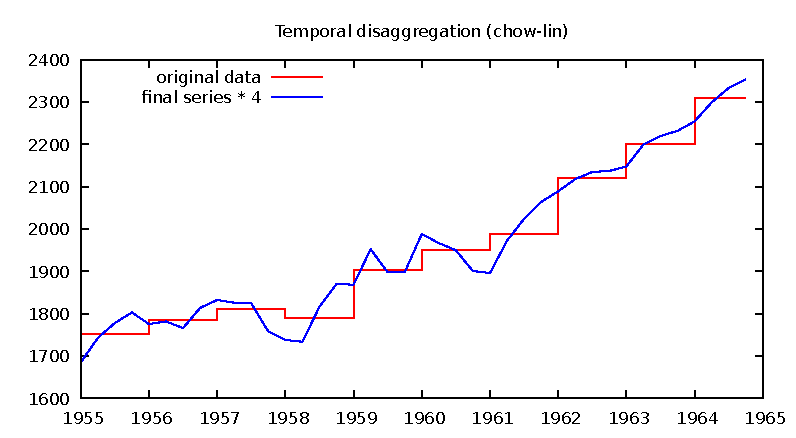
\includegraphics{figures/gnpa}
  \caption{Example output from plot option, showing annual GNP (red)
    and quarterly final series (blue) using quarterly industrial
    production as indicator.}
  \label{fig:gnpa}
\end{figure}

If there are many observations, the two lines may appear virtually
coincident. In that case one can see what's going on in more detail by
exploiting the ``Zoom'' functionality of the plot, which is accessed
via the right-click menu in the plot window.

\section{Multiple low-frequency series}
\label{sec:tdisagg-multi}

We now return to a point mentioned in section~\ref{sec:tdisagg-nd},
namely, that $\Yb$ may be given as a $T \times g$ matrix with $g > 1$,
or a list of $g$ series. This means that a single call to
\texttt{tdisagg} can be used to process several input series (``batch
processing''), in which case the return value is a matrix with $(s
\cdot T + m)$ rows and $g$ columns.

There are some restrictions. First and most obviously, a single call
to \texttt{tdisagg} implies a single selection of ``indicators'' or
``related series'' ($\Xb$) and a single selection of options
(aggregation type of the data, deterministic terms, disaggregation
method, and so on). So this possibility will be relevant only if you
have several series that ``want the same treatment.'' In addition, if
$g > 1$ the \texttt{plot} and \texttt{verbose} options are ignored and
the \texttt{results} bundle is not filled; if you need those features
you should supply a single series or vector in $\Yb$.

The advantage of batch processing lies in the spreading of fixed
computational cost, leading to shorter execution time. However, the
relative importance of the fixed cost differs substantially according
to the disaggregation method. For the Chow--Lin methods the fixed cost
is relatively small and so little speed-up can be expected, but for
the Denton methods it dominates, and (in our testing) you can process
$g > 1$ series in little more time than it takes to process a single
series.

As they say, ``Your mileage may vary,'' but if you have a large number
of series to be disaggregated via one of the Denton methods you may
well find it much faster to use the batch facility of
\texttt{tdisagg}.

\section{Examples}
\label{sec:tdisagg-examples}

Listing~\ref{listing:tdscript} shows an example of usage and its
output. The data are drawn from the St Louis Fed; we disaggregate
quarterly GDP to monthly with the help of industrial production and
payroll employment, using the default Chow--Lin method.

Several other example scripts are available from
\url{http://gretl.sourceforge.net/tdisagg/}.

\begin{script}[htbp]
  \caption{Example of \texttt{tdisagg} usage}
  \label{listing:tdscript}
 Input:
\begin{scodebit}
### Traditional Chow-Lin: y is a series with repetition
### and X is a list of series. This corresponds to case 4(a)
### as described in section 9.3 of the documentation above.
###

# ensure that no data are in place
clear
# open gretl's St Louis Fed database
open fedstl.bin
# import two monthly series
data indpro payems
# import quarterly GDP (values are repeated)
data gdpc1

# restrict sample to complete data
smpl --no-missing

# disaggregate GDP from quarterly to monthly, using
# industrial production and payroll employment as indicators
scalar s = 3
list X = indpro payems
series gdpm = tdisagg(gdpc1, X, s, _(verbose=1, aggtype="sum"))
\end{scodebit}
  Output:
\begin{scodebit}
Aggregation type sum
GLS estimates (chow-lin) T = 294
Dependent variable: gdpc1

             coefficient    std. error    t-ratio   p-value 
  ----------------------------------------------------------
  const      312.394       263.372         1.186    0.2365  
  indpro      10.9158        1.75785       6.210    1.83e-09 ***
  payems       0.0242860     0.00171935   14.13     7.39e-35 ***

  rho = 0.999, SSR = 51543.9, lnl = -1604.98

Generated series gdpm (ID 4)
\end{scodebit}
\end{script}

